%!TEX root=./main.tex

\section{Evaluation}\label{sec:experiment}


\begin{comment}
\paragraph*{Experimental Setup}
    We conducted all experiments on a Dell Latitude 5450 system running
a custom Debian-based distribution with an Intel Core Ultra 5 135H CPU
(18 cores @ 4.60 GHz) and 32GB of RAM.
%
We set a timeout of 60 minutes and a memory limit of 512MB
(denoted by \timeout\ and \oom). 
\MZ{do we need this? Experiments were run on my local Mac}
\RM{if you ran on your laptop, why not give the specs of your laptop?
Where is OOM and timeout used later?} \MZ{that was why I asked, we ran this simulator and we didn't report performance }

\end{comment}





\subsubsection*{Implementation and Setup}

We implemented \textbf{Algorithm S} in a tool called \testor. 
It is built on top of \jmc~\cite{jmc}, an implementation of \trust for Java programs~\cite{condpor}.
%%(details on the implementation of the \testor algorithm are provided in \cref{app:testor-impl}). 
For our evaluation, we also developed an ``offline'' version of \testor that runs \textbf{Algorithm S} 
on the tree ($\mathcal{D}(P)$) by running \jmc until completion and logging the events.
% Since tree logger in \jmc defers state transitions whenever a state has a unique $\fwdtikz$ successor and only materializes states at branching points and $\bwdtikz$, \MZ{@mohammad, is there anything to be addressed with the online implementation?} \MO{I've added a section in the appendix to discuss the implementation.}
% the resulting tree model is more compact than one in which every event is treated as a separate state transition.
%We apply offline \testor to this logged tree, exactly 
% simulating the behavior it would have when embedded in a stateless \dpor exploration of $\mathcal{D}(P)$ 
% while isolating its statistical properties from runtime overheads.
%
%For our evaluation, we additionally developed an ``offline'' variant of \testor that operates on the pre-collected $\mathcal{D}(P)$, obtained by running \jmc to completion.
The offline variant simulates exactly the behavior of \testor as it would operate when embedded in a stateless \dpor exploration of $\mathcal{D}(P)$, thereby isolating its statistical properties from runtime overheads.

As a baseline, we also implemented \textbf{Algorithm P} directly within \jmc.
However, we found that the variance of this algorithm is so large that, in all of our experiments, the estimates never converge into a meaningful value.
All experiments were conducted on a MacBook Pro equipped with 34GB of RAM and an M3 chip.

\subsubsection*{Benchmarks}
Our benchmark set consists of handcrafted (\textsc{IncNTest}, \textsc{FineCounter}) and SV-COMP-\texttt{pthread} \cite{svcomp} benchmarks (\textsc{Big0}, \textsc{Fib1}, \textsc{Sigma}, \textsc{SVQueue2}, \textsc{SVQueue3}, and \textsc{SVStack2}),
  textbook concurrent lists/stacks/queues (\textsc{CoarseList} \cite{book:herlihy-shavit}, \textsc{FineList} \cite{finelist}, \textsc{OptList} \cite{book:herlihy-shavit}, \textsc{UbQueue} \cite{book:herlihy-shavit}, 
  \textsc{LbQueue} \cite{book:herlihy-shavit}, and \textsc{AgmStack} \cite{agmstack}), and real-world data structures such as \textsc{TimestampStack} \cite{timestamped-stack}.



\subsection{Overview }
We consider the following two configurations in our evaluation.

 
\begin{enumerate}[label=\textbf{(\Alph*)}, leftmargin=2em]
\item \label{phase:online}
We evaluate the practical potential of \testor by running it on a representative set of benchmarks with varying workloads.
For each benchmark suite, we run online \testor for 1 minute and 5 minutes, assess the accuracy of the resulting estimates, and compare its running time against that of \jmc run to completion or until timeout.
% \item \label{phase:acp}\textbf{Approximate Counting Problem.}In this part, we ask how quickly do our estimators converge in practical benchmarks and how well the estimators scale as the workload (and consequently the state space) increases.
  %
\item \label{phase:acp} We then conduct a principled evaluation of the offline implementation. The offline setting enables a cleaner experimental setup, isolates the estimator from runtime-dependent effects, and improves reproducibility. We run the estimator on $\mathcal{D}(P)$ until it converges to a value close to the ground truth, and examine how its behavior varies across different budget settings.

%  We evaluate evaluating \testor and \pestor across synthetic benchmarks consists of handcrafted (IncNTest, FineCounter) and SV-COMP \texttt{pthread} category \cite{svcomp} benchmarks (Big0, Fib1, Sigma, SV Queue2, SV Queue3, and SV Stack2),
%  classic concurrent stacks/queues (CoarseList\cite{book:herlihy-shavit}, FineList\cite{finelist}, OptList\cite{book:herlihy-shavit}, UbQueue\cite{book:herlihy-shavit}, LbQueue\cite{book:herlihy-shavit}, and AgmStack\cite{agmstack}), and real-world data structures (timestamped stacks\cite{timestamped-stack}). 
%  We examine practical convergence on standard concurrent patterns.

  %\item \label{phase:trust-cost}\textbf{\jmc\ Cost Estimation.}In this part, we use \testor to evaluate the cost of model checking: is \testor effective in estimating the total cost of exploration?
\end{enumerate}  
% A word is in order to distinguish the two questions.While $C(P)$ is a \emph{lower bound} on the work that a model checker must do, in practice, model checkers perform additional work,e.g., by checking consistency of execution graphs and exploring ``blocked'' executions.The latter arise in model checking programs in the presence of blocking synchronization primitives such as spinloops, await loops, and confirmation CAS.A typical approach is to replace the looping behavior by an \emph{assume} statement, which proceeds by trying to acquire a lock and assuming that it succeeds \cite{awamoche}.As part of the exploration, this can lead to blocked executions in which the assume fails.Such executions do not correspond to genuine program behaviors but must be considered as part of the cost of exploration.


%Since the number of maximal executions is a lower bound on the work that any \dpor-based model checker must do, we can be more accurate when given the specific model checker \jmc by estimating with a better proxy for its computational cost. In practice, \jmc also spends time checking consistency predicate over executions and exploring executions that are not maximal. More importantly, 
%In the context of stateless \dpor-based model checking, spinloops, await loops, and confirmation-CAS loops are compiled into 
%\(\assume(\varphi)\) statements( while lock acquisitions and releases can be handled differently). In certain circumstances, the model checker marks the corresponding thread as permanently blocked, and may %treat that execution graph as maximal even though, in general, such a blocked execution does not correspond to a genuine program behavior (there may exist other schedules in which the thread is not blocked).
%Considering existence optimization to avoid the exploration of unnecessary blocked executions or to perform in-place commutation\cite{awamoche}, no \dpor technique currently exists that can fully avoid %exploring blocked executions. Thus, if \(X(P)\) is the set of all maximal execution graphs explored by any \dpor-based model checker, then \(C(P) \subseteq X(P)\).Since our evaluation setup guarantees that %the offline simulation exactly matches the estimator’s online behavior, we exclude benchmarks whose search space is dominated by blocked executions from Configuration \ref{phase:acp} for clarity of analysis, but do %include them in this phase. Moreover, in addition to benchmarks we used in Configuration \ref{phase:acp}, we evaluate over Treiber stack\cite{treiberstack}, MsQueue\cite{msqueue}, TtasLock\cite{ttaslock}, MPMC %Queue\cite{gator}, Linux-r-w-lock\cite{gator}, and Elimination-backoff Stack\cite{ebstack}.
%Therefore, to capture this more realistic notion of cost, we specialize \testor to estimate the computational \textbf{cost} of \jmc by charging work to every explored execution including the blocked ones in 
%a way that emulates the cost incurred by \jmc.

\begin{table}[tbp]
\centering
\tiny



\begin{tabular}{llcccc}
\toprule
Benchmark & Param & Est.\ @1m & Est.\ @5m & \jmc count & \jmc status \\
\midrule
\multirow{3}{*}{CoarseList} & 8 & $(4.63 \pm 1.49) \times 10^{4}$ & $(4.13 \pm 0.77) \times 10^{4}$ & $4.03 \times 10^{4}$ & 1m 34s \\
 & 9 & $(6.72 \pm 5.65) \times 10^{5}$ & $(4.12 \pm 2.76) \times 10^{5}$ & $3.63 \times 10^{5}$ & 14m 11s \\
 & 10 & $(1.93 \pm 0.98) \times 10^{6}$ & $(2.12 \pm 0.54) \times 10^{6}$ & $>1.13 \times 10^{6}$ & TO at 1h \\
\midrule
\multirow{3}{*}{Fib1} & 10 & $(1.84 \pm 0.27) \times 10^{5}$ & $(1.87 \pm 0.06) \times 10^{5}$ & $1.85 \times 10^{5}$ & 6m 46s \\
 & 11 & $(6.93 \pm 1.10) \times 10^{5}$ & $(7.02 \pm 0.51) \times 10^{5}$ & $7.05 \times 10^{5}$ & 27m 15s \\
 & 12 & $(2.62 \pm 0.09) \times 10^{6}$ & $(2.61 \pm 0.16) \times 10^{6}$ & $>1.50 \times 10^{6}$ & TO at 1h  \\
\midrule
\multirow{3}{*}{FineCounter} & 11 & $(9.84 \pm 1.87) \times 10^{4}$ & $(1.21 \pm 0.11) \times 10^{5}$ & $8.64 \times 10^{4}$ & 2m 57s \\
 & 12 & $(7.83 \pm 3.12) \times 10^{5}$ & $(5.75 \pm 1.49) \times 10^{5}$ & $5.18 \times 10^{5}$ & 18m 3s \\
 & 13 & $(3.35 \pm 1.87) \times 10^{6}$ & $(3.78 \pm 1.48) \times 10^{6}$ & $>1.60 \times 10^{6}$ & TO at 1h  \\
\midrule
\multirow{3}{*}{FineList} & 8 & $(5.60 \pm 0.76) \times 10^{4}$ & $(4.37 \pm 0.37) \times 10^{4}$ & $4.03 \times 10^{4}$ & 2m 16s \\
 & 9 & $(3.25 \pm 2.55) \times 10^{5}$ & $(3.10 \pm 0.67) \times 10^{5}$ & $3.63 \times 10^{5}$ & 22m \\
 & 10 & $(3.13 \pm 0.67) \times 10^{5}$ & $(3.58 \pm 2.30) \times 10^{6}$ & $>8.85 \times 10^{5}$ & TO at 1h  \\
\midrule
\multirow{3}{*}{IncNTest} & 5 & $(1.43 \pm 0.06) \times 10^{4}$ & $(1.43 \pm 0.03) \times 10^{4}$ & $1.44 \times 10^{4}$ & 19s \\
 & 6 & $(4.96 \pm 0.88) \times 10^{5}$ & $(5.68 \pm 1.00) \times 10^{5}$ & $5.18 \times 10^{5}$ & 5m 15s \\
 & 7 & $(2.41 \pm 0.56) \times 10^{7}$ & $(2.42 \pm 0.51) \times 10^{7}$ & $>5.18 \times 10^{6}$ & TO at 1h  \\
\midrule
\multirow{3}{*}{OptList} & 4 & $(1.78 \pm 0.05) \times 10^{3}$ & $(1.77 \pm 0.05) \times 10^{3}$ & $1.69 \times 10^{3}$ & 15s \\
 & 5 & $(4.59 \pm 1.92) \times 10^{5}$ & $(4.83 \pm 1.11) \times 10^{5}$ & $4.57 \times 10^{5}$ & 16m 45s \\
 & 6 & $(1.94 \pm 3.20) \times 10^{8}$ & $(3.27 \pm 4.75) \times 10^{8}$ & $>1.16 \times 10^{6}$ & TO at 1h  \\
\midrule
\multirow{3}{*}{SVStack2} & 10 & $(6.73 \pm 1.18) \times 10^{4}$ & $(6.75 \pm 0.11) \times 10^{4}$ & $6.87 \times 10^{4}$ & 3m 15s \\
 & 11 & $(2.37 \pm 0.54) \times 10^{5}$ & $(2.53 \pm 0.30) \times 10^{5}$ & $2.42 \times 10^{5}$ & 11m 39s \\
 & 12 & $(7.60 \pm 0.99) \times 10^{5}$ & $(8.91 \pm 0.52) \times 10^{5}$ & $8.59 \times 10^{5}$ & 43m 39s \\
\midrule
\multirow{3}{*}{SVQueue2} & 9 & $(5.07 \pm 0.29) \times 10^{4}$ & $(4.73 \pm 0.19) \times 10^{4}$ & $4.86 \times 10^{4}$ & 4m 34s \\
 & 10 & $(1.88 \pm 0.22) \times 10^{5}$ & $(1.92 \pm 0.20) \times 10^{5}$ & $1.85 \times 10^{5}$ & 19m 38s \\
 & 11 & $(6.63 \pm 2.31) \times 10^{5}$ & $(7.38 \pm 0.88) \times 10^{5}$ & $>4.89 \times 10^{5}$ & TO at 1h  \\

\midrule
\multirow{3}{*}{SVQueue3}  & 15 & $(8.87 \pm 1.15) \times 10^{4}$ & $(1.13 \pm 0.11) \times 10^{5}$ & $1.09 \times 10^{5}$ & 8m 21s \\
 & 16 & $(2.05 \pm 0.85) \times 10^{5}$ & $(2.25 \pm 0.50) \times 10^{5}$ & $2.18 \times 10^{5}$ & 17m 5s \\
 & 17 & $(4.25 \pm 2.08) \times 10^{5}$ & $(5.43 \pm 2.74) \times 10^{5}$ & $4.37 \times 10^{5}$ & 36m 31s \\
\midrule
\multirow{3}{*}{UBQueue} & 9 & $(4.60 \pm 0.50) \times 10^{4}$ & $(4.61 \pm 0.10) \times 10^{4}$ & $4.61 \times 10^{4}$ & 1m 23s \\
 & 10 & $(5.01 \pm 1.86) \times 10^{5}$ & $(4.58 \pm 0.20) \times 10^{5}$ & $4.61 \times 10^{5}$ & 13m 16s \\
 & 11 & $(2.28 \pm 0.92) \times 10^{6}$ & $(2.98 \pm 0.30) \times 10^{6}$ & $>1.85 \times 10^{6}$ & TO at 1h  \\
 \midrule
 \multirow{3}{*}{LBQueue} & 13 & $(1.03 \pm 0.88) \times 10^{5}$ & $(6.23 \pm 0.76) \times 10^{4}$ & $6.91 \times 10^{4}$ & 3m 52s \\
 & 14 & $(2.48 \pm 1.12) \times 10^{5}$ & $(3.49 \pm 1.03) \times 10^{5}$ & $3.46 \times 10^{5}$ & 19m 45s \\
 & 15 & $(5.98 \pm 2.57) \times 10^{5}$ & $(1.65 \pm 1.45) \times 10^{6}$ & $>9.69 \times 10^{5}$ & TO at 1h  \\
 \midrule
\multirow{3}{*}{AgmStack} & 5 & $(6.25 \pm 0.36) \times 10^{3}$ & $(6.15 \pm 0.15) \times 10^{3}$ & $6.23 \times 10^{3}$ & 19s \\
 & 6 & $(5.14 \pm 1.25) \times 10^{5}$ & $(4.28 \pm 0.76) \times 10^{5}$ & $4.48 \times 10^{5}$ & 11m 41s \\
 & 7 & $(4.36 \pm 2.75) \times 10^{7}$ & $(5.07 \pm 1.52) \times 10^{7}$ & $>1.87 \times 10^{6}$ & TO at 1h  \\
 \midrule
\multirow{3}{*}{Sigma} & 4 & $(1.49 \pm 0.09) \times 10^{4}$ & $(1.40 \pm 0.05) \times 10^{4}$ & $1.38 \times 10^{4}$ & 20s \\
 & 5 & $(4.36 \pm 4.00) \times 10^{6}$ & $(1.64 \pm 0.41) \times 10^{6}$ & $1.73 \times 10^{6}$ & 21m 27s \\
 & 6 & $(2.61 \pm 2.57) \times 10^{8}$ & $(4.16 \pm 5.21) \times 10^{8}$ & $>3.85 \times 10^{6}$ & TO at 1h  \\
 \midrule
\multirow{3}{*}{TimeStampStack} & 3 & $(2.94 \pm 0.11) \times 10^{2}$ & $(2.90 \pm 0.05) \times 10^{2}$ & $2.91 \times 10^{2}$ & 12s \\
 & 4 & $(3.34 \pm 0.60) \times 10^{4}$ & $(4.71 \pm 0.60) \times 10^{4}$ & $3.26 \times 10^{4}$ & 1m 54s \\
 & 5 & $(1.41 \pm 2.29) \times 10^{7}$ & $(3.50 \pm 1.09) \times 10^{6}$ & $>7.76 \times 10^{5}$ & TO at 1h  \\
\bottomrule
\end{tabular}
\vspace{7pt}
\caption{Results of the online \testor with stochastic enumeration budget of 20 under fixed 1-minute and 5-minute time constraints, compared with the corresponding \jmc runs. For each benchmark and parameter, each estimator entry reports the mean and standard deviation over 5 independent runs. The \jmc \textit{count} column reports the number of executions explored by \jmc, which is exact when the run finishes and partial when the run times out. The \jmc \textit{status} column reports the \jmc execution time, or indicates a timeout when the run does not finish within the time limit.}
\label{tab:online-estimator-results}
\end{table}


\subsection{Configuration \ref{phase:online}: Effectiveness of \testor}

In this configuration, we evaluate \testor as a tool for estimating the state space of a program.

\subsubsection*{Setup}

A practical use case for \testor is as a lightweight budgeting tool: one first runs the estimator for a short period, and then uses the resulting estimate to inform how long the model checker should continue running.
Accordingly, in this configuration, we run \testor for 1 minute and 5 minutes, and run \jmc with a 1-hour time limit.

We consider a set of standard concurrent benchmarks whose workload scales with input parameters, such as the number of workers or the number of operations.
For each benchmark, we select three workload configurations: one for which the model checker finishes comfortably within the time limit, one expected to be close to the largest workload the model checker can still handle within the time limit, and one for which the model checker is unlikely to terminate within the time limit.
For each benchmark–workload configuration, we run \testor five times and record the mean estimate, as well as the standard deviation.
We adopt a stochastic enumeration budget of $\mathcal{B} = 20$, informed by the findings of our study in Configuration~\ref{phase:acp}.

\subsubsection*{Observations}
Table~\ref{tab:online-estimator-results} reports the performance of \testor under fixed one-minute and five-minute budgets, alongside the corresponding model-checking runs. For each benchmark and parameter setting, each estimator entry reports the mean and standard deviation over 5 independent runs. The \jmc \emph{count} column gives the number of executions explored by \jmc: this is exact when \jmc terminates within the time limit, and partial when the run times out. The \jmc \emph{status} column reports either the wall-clock time of the completed model-checking run or the timeout status.
Overall, \testor yields encouraging results. On configurations for which \jmc terminates and the exact count is known, 99 out of 150 1-minute runs and 113 out of 150 5-minute runs fall within 80\%–120\% of the exact count.
On the subset of non-timeout configurations whose exact \jmc runs take more than 5 minutes, 47 out of 85 1-minute runs and 61 out of 85 5-minute runs fall within 80\%–120\% of the exact count. This suggests that even a short fixed budget often suffices to obtain a useful estimate, while a 5-minute budget yields a meaningful improvement in fine-grained accuracy. As expected, 1-minute estimates exhibit higher standard deviations than their 5-minute counterparts.
For the smallest configurations, exhaustive exploration finishes before the one minute and five minute deadline; however, there is no a priori way to predict that this will happen other than by computing estimates.

The table further illustrates that the practical value of  \testor extends beyond predicting the final count: it also reveals how difficulty scales across neighboring workload configurations. For instance, on \textsc{CoarseList}, the estimated count increases by only a factor of approximately five from parameter~9 to parameter~10. Although the parameter-10 model-checking run times out, this estimate suggests that the exact run may still be feasible within a few hours. Moreover, the partial count at timeout already covers roughly half of the estimated total, providing a meaningful measure of progress. In contrast, for \textsc{OptList}, the estimator predicts a jump from only hundreds of thousands of executions to hundreds of millions. This indicates a much sharper scalability cliff: even substantially extending the execution time is unlikely to make the larger instance tractable, and the roughly one million executions explored before timeout may represent only a negligible fraction of the total space.

We note that the issue of variance is not fully mitigated.
For example, one configuration of \textsc{CoarseList} exhibits an unusually large standard deviation. 
Upon inspection, this is caused not by pervasive instability across all repeated runs, but by a single outlying run among the five repetitions. 
%This suggests that, for certain program structures,  
%\testor may occasionally produce rare but substantial deviations even under identical time budgets.
We also observe that when the estimator returns a large estimate, the standard deviation tends to be larger as well, which is expected. 
A short runtime is unlikely to suffice for accurate estimation when the underlying search space is inherently enormous. Nevertheless, in such cases, even obtaining the correct order of magnitude is already very useful.


%!TEX root=./main.tex

\begin{table}[t]
  \centering
  \tiny
  \begin{tabular}{@{} l l S[scientific-notation=true] S[table-format=1.2] l @{}}
    \toprule
    \textbf{Concurrent Structures} & \textbf{Estimator} & \textbf{Relative Error} & \textbf{Success Ratio} & \textbf{Trials} \\
    \midrule

   \multirow{4}{*}{\makecell[l]{CoarseList\\ Insertion threads=9\\ Executions = \num{362880}}} &  B=1 & \num{1.42} & \num{0} & (failed) \\
    &  B=5      & \num{0.25} & \num{0.20} & (failed) \\
    &  B=20     & \num{0.0647} & {1 \ding{51}} & \num{187} \\
    &  B=50     & \num{0.0271} & {1\ding{51}} & \num{125} \\
    \midrule
    \multirow{4}{*}{\makecell[l]{FineList\\ Insertion threads=9\\ Executions = \num{362880}}} &  B=1 & \num{1.42} & \num{0} & (failed) \\
    &  B=5      & \num{0.25} & \num{0.20} & (failed) \\
    &  B=20     & \num{0.0647} & {1\ding{51}} & \num{187} \\
    &  B=50     & \num{0.0271} & {1\ding{51}} & \num{125} \\
    \midrule
     \multirow{4}{*}{\makecell[l]{OptList\\ Insertion threads=3\\ Deletion threads=2\\ Executions = \num{456995}}} & B=1 & \num{0.784} & \num{0} & (failed) \\
    &  B=5      & \num{0.32} & {\num{0.60}\,\ding{51}} & \num{1156} \\
    &  B=20     & \num{0.371} & {\num{0.80}\,\ding{51}} & \num{794} \\
    &  B=50     & \num{0.0851} & {1\ding{51}} & \num{210} \\
    \midrule
    \multirow{4}{*}{\makecell[l]{UbQueue\\ Insertion threads=5\\ Deletion threads=5\\Executions = \num{460800}}} &  B=1             & \num{0.217} & \num{0.40} & (failed) \\
    &  B=5            & \num{0.0654} & {1\ding{51}} & \num{350} \\
    &  B=20           & \num{0.0303} & {1\ding{51}} & \num{311} \\
    &  B=50           & \num{0.00845} & {1\ding{51}} & \num{126} \\ 
    \midrule
        \multirow{4}{*}{\makecell[l]{LbQueue\\  Enqueue threads=14\\Executions = \num{345600}}} &  B=1              & \num{0.787} & \num{0} & (failed) \\
    &  B=5             & \num{0.191} & {\num{0.60}\,\ding{51}}  & \num{1097} \\
    &  B=20            & \num{0.0604} & {1\ding{51}} & \num{165} \\
    &  B=50            & \num{0.0408} & {1\ding{51}} & \num{197}  \\ 
    \midrule
\multirow{4}{*}{\makecell[l]{AmgStack\\ Pusher threads=3\\ Poper thread threads=3\\ Exeuctions = \num{447576}}} & B=1 & \num{0.509} & \num{0.00} & (failed) \\
    &B=5      & \num{0.191} & {\num{0.60}\,\ding{51}}  & \num{1005} \\
    &  B=20     & \num{0.0469} & {1\ding{51}} & \num{456} \\
    & B=50     & \num{0.0429} & {1\ding{51}} & \num{357} \\
    \midrule
    
\multirow{4}{*}{\makecell[l]{TimeStampStack\\ Pusher threads=2\\ Poper thread threads=2\\ Executions = \num{32648}}} &   B=1 & \num{0.395} & \num{0.00} & (failed) \\
    &  B=5      & \num{0.21} & {\num{0.60}\,\ding{51}} & \num{1100} \\
    &  B=20     & \num{0.0376} & {1\ding{51}} & \num{479} \\
    &  B=50     & \num{0.0362} & {1\ding{51}} & \num{286} \\
    \bottomrule



  \end{tabular}

  \vspace{0.1in}
  \caption{Concurrent data structure benchmarks for estimator evaluation on  \textbf{maximal executions}. Columns (left→right): benchmark info, which contains input detail and total complete execution number; estimator configuration; average relative error after 2000 trials; success ratio (fraction of 5 seeds that converge within the 80–120\% band); and average trials to converge across the successful seeds (reported only if success ratio$\geq 0.6$; otherwise shown as “failed”). }
    \label{tab:convergence}

\end{table}


%!TEX root=./main.tex

\begin{table}[t]
  \centering
  \tiny
  \begin{tabular}{@{} l l S[scientific-notation=true] S[table-format=1.2] l @{}}
    \toprule
    \textbf{Synthetic Benchmarks} & \textbf{Estimator} & \textbf{Relative Error} & \textbf{Success Ratio} & \textbf{Trials} \\
    \midrule
\multirow{5}{*}{\makecell[l]{IncNTest\\  Incrementor threads=6\\ Executions = \num{518400}}} &   B=1 & \num{0.408} & \num{0.20} & (failed) \\
    & B=5      & \num{0.206} & {\num{0.60}\,\ding{51}}  & \num{575} \\
    &  B=20     & \num{0.256} & {1\ding{51}} & \num{909} \\
    &  B=50     & \num{0.0535} & {1\ding{51}} & \num{560} \\
    \midrule
\multirow{4}{*}{\makecell[l]{Big0\\ Executions = \num{69112}}} &   B=1              & \num{0.0333} & {1\ding{51}}& \num{159} \\
    &  B=5             & \num{0.0068} & {1\ding{51}} & \num{151} \\
    &  B=20            & \num{0.00767} & {1\ding{51}} & \num{112} \\
    &  B=50            & \num{0.00231} & {1\ding{51}} & \num{106}  \\
    \midrule
\multirow{4}{*}{\makecell[l]{FineCounter\\   Threads=12\\ Executions = \num{518400}}} &   B=1 & \num{0.651} & \num{0} & (failed) \\
    &  B=5      & \num{0.481} & \num{0.20} & (failed) \\
    &  B=20     & \num{0.0923} & {1\ding{51}} & \num{192} \\
    &  B=50     & \num{0.0454} & {1\ding{51}} & \num{239} \\
  
    \midrule
    \multirow{4}{*}{\makecell[l]{Fib1\\   operations=11\\ Executions = \num{705432}}} &    B=1              & \num{2.9} & \num{0.20} & (failed) \\
    &  B=5             & \num{0.0951} &  {1\ding{51}} & \num{570} \\
    &  B=20            & \num{0.0402} &  {1\ding{51}} & \num{184} \\
    &    B=50            & \num{0.0204} &  {1\ding{51}} & \num{136} \\ 
    \midrule
    \multirow{4}{*}{\makecell[l]{Sigma\\   operations=5\\ Executions = \num{1728000}}} &   B=1              & \num{0.53} & \num{0} & (failed) \\
    &  B=5             & \num{2.68} & {\num{0.60}\,\ding{51}} & \num{1342} \\
    &  B=20            & \num{0.616} &  {1\ding{51}} & \num{1022} \\
    &  B=50            & \num{0.108} & {\num{0.80}\,\ding{51}} & \num{552} \\ 
  
    \midrule
      \multirow{4}{*}{\makecell[l]{SV Queue2\\   Operations=10\\ Executions = \num{184756}}} &  B=1 & \num{0.651} & \num{0} & (failed) \\
    &  B=5      & \num{0.105} &  {1\ding{51}} & \num{395} \\
    &  B=20     & \num{0.0319} &  {1\ding{51}} & \num{174} \\
    &  B=50     & \num{0.0104} &  {1\ding{51}} & \num{127} \\
     \midrule
        \multirow{4}{*}{\makecell[l]{SV Queue3\\   Operations=17\\ Executions = \num{436728}}} & B=1      & \num{0.956} & \num{0.00} & (failed) \\
    & B=5      & \num{0.396} & \num{0.40} & (failed) \\
    & B=20     & \num{0.0696} &  {1\ding{51}} & \num{715} \\
    & B=50     & \num{0.0162} &  {1\ding{51}} & \num{140} \\
     \midrule
      \multirow{4}{*}{\makecell[l]{SV Stack2\\   Operations=11\\ Executions = \num{241616}}} &  B=1 & \num{0.408} & \num{0} & (failed) \\
    &  B=5      & \num{0.266} &  {1\ding{51}} & \num{791} \\
    &  B=20     & \num{0.0314} &  {1\ding{51}} & \num{259} \\
    &  B=50     & \num{0.0306} &  {1\ding{51}} & \num{135} \\
    \bottomrule




  \end{tabular}

  \vspace{0.1in}
  \caption{Synthetic benchmarks for estimator evaluation on \textbf{maximal executions}. Columns (left→right): benchmark info; estimator configuration; average relative error after 2000 trials; success ratio (fraction of 5 seeds that converge within the 80–120\% band); and average trials to converge across the successful seeds (reported only if success ratio$\geq 0.6$; otherwise shown as “failed”). }
    \label{tab:synthtic_converge}

\end{table}


\subsection{Configuration \ref{phase:acp}: Convergence of Estimation
}

%Although unbiased estimators converge to the expected value, this guarantee is often meaningless in practice: high variance can lead to extreme instability or even non-convergence under any practical finite budgets.
% Thus, our first question is whether our estimators exhibit practical convergence within a modest sampling budget when estimating program behavior spaces.

We use the offline implementation to  explore the convergence behavior of \testor's estimation in a principled manner.

\subsubsection*{Setup}
In this configuration, we consider offline-\testor has succeeded if its estimate converges to a range around the real count. 
Specifically, we declare convergence when the running mean of offline-\testor enters the $\pm20\%$ relative error band and remains within it for a stability window of 
$50$ iterations, while also satisfying a flatness condition: the moving average changes by less than a $2\%$ relative threshold over a stability window of 100 iterations.
We evaluate four configurations of offline-\testor with stochastic enumeration budgets $\mathcal{B} \in \{1, 5, 20, 50\}$. 
Each configuration is executed for a sequence of $2000$ runs, and to account for randomness, each sequence is repeated with five independent random seeds. 
A configuration is deemed to successfully converge if it converges under at least three of the five seeds. 
To assess the effectiveness of our estimators, we focus on two metrics:
\begin{enumerate}
    \item \emph{Relative error after 2000 runs}, computed as $\text{estimated count} / \text{exact count}$; and
    \item \emph{Trials to convergence}, reported only when a configuration converges on a given benchmark and averaged over the seeds for which convergence was achieved.
\end{enumerate}

\subsubsection*{Benchmarks}

For this evaluation configuration, we study \testor on 15 benchmarks: the same benchmark suite used in Configuration~\ref{phase:online}, plus one additional benchmark (Big0) that is small and does not have a tunable parameter, and was therefore not included in Configuration~\ref{phase:online}.
 
The first seven benchmarks (presented in \cref{tab:convergence}) correspond to typical uses of concurrent data structures, 
including \textsc{CoarseList}, \textsc{FineList}, \textsc{OptList}, \textsc{UbQueue}, \textsc{LbQueue}, \textsc{AMGStack}, and \textsc{TimestampStack}. 
These programs exhibit high thread contention, yielding large and complex behavior spaces. 
The remaining eight (presented in \cref{tab:synthtic_converge}) are synthetic benchmarks designed to isolate specific concurrency 
patterns and stress particular aspects of the estimators’ convergence behavior.
%We omitted the others because they are dominated by blocked executions---we will return to them in Configuration (B) \MO{I think this citation is wrong}.

\subsubsection*{Results Summary}

\Cref{tab:convergence} and \ref{tab:synthtic_converge} present the results of the evaluation. 
%For each benchmark, we first report the details of the program. 
For each estimator configuration, we report (i) the average relative error after 2,000 trials, averaged over all 5 seeds, 
(ii) the success ratio (i.e., the fraction of seeds that satisfy the convergence criterion), and 
(iii) when this ratio exceeds 0.6 (at least 3 out of 5 seeds), the average number of trials-to-convergence over the converged seeds (rounded to int).

We note that the baseline \textbf{Algorithm P} failed to converge on every benchmark.

% RM: This is not unexpected, right? THe number depends on the concurrency structure of the test
%We also note that different benchmarks can induce the same underlying tree. 
%For instance, our \textsc{CoarseList} and \textsc{FineList} benchmarks, although implemented as different data structures, yield exactly the same estimates when we run them under the same random seeds.

\begin{description}
    \item[Convergence:] Positively, we observe offline-\testor with budgets of 20 and 50 converges on all benchmarks within a very small 
    number of trials--—typically a few hundred--—even when the underlying behavior space is much larger, 
    ranging from 30 thousand up to 1.7 million. We therefore believe that our evaluation demonstrates the practicality of our estimator.
    On the other hand, offline-\testor with a budget of 1 (\textbf{Algorithm T}) failed to converge on all benchmarks except Big0.
    \item[Relative Error:] Offline-\testor with budgets of 20 and 50 generally yields very small relative errors after 2000 runs. While a budget of 50 does not show a clear advantage in achieving convergence compared to a budget of 20, it does provide a noticeable improvement in the final relative error. We also observe that, for most benchmarks, whenever a configuration reported convergence, the relative error induced by the configuration remains well within the $20\%$ band.
    %%indicating that our convergence criterion is appropriately chosen. 
\end{description}

\subsection{Configuration~\ref{phase:acp}: Scaling with Budget}
%\subsubsection*{Scaling with Workload}Based on the previous result, a budget of 20 appears sufficient for our purpose. It offers comparable accuracy (converged for all benchmarks with success ratio  while requiring fewer computational resources compared to budget 50, so we use it as the default setting in the subsequent analysis.In this section, we first study its expected scaling behavior by examining how convergence evolves as the workload of the same benchmark grows.We examine several representative benchmarks under different workloads, varying the number of threads and operations to observe how the estimator’s convergence time scales with the growth of the space. We continue running with 2,000 runs and report the average number of trials required for convergence. As shown in Figure \ref{fig:workload}, the estimator converges quickly on small search spaces and continues to scale gracefully as the search space grows. Even for large spaces, the increase in convergence time remains sublinear, indicating that the estimator maintains efficiency across several orders of magnitude. More importantly, we find that for large workload, the number of trials required for our estimator to converge is typically at least thousands of times smaller than the total number of behaviors, demonstrating that it achieves stable estimates after exploring only a minute fraction of the search space. %

\begin{figure}[t]
  \centering
  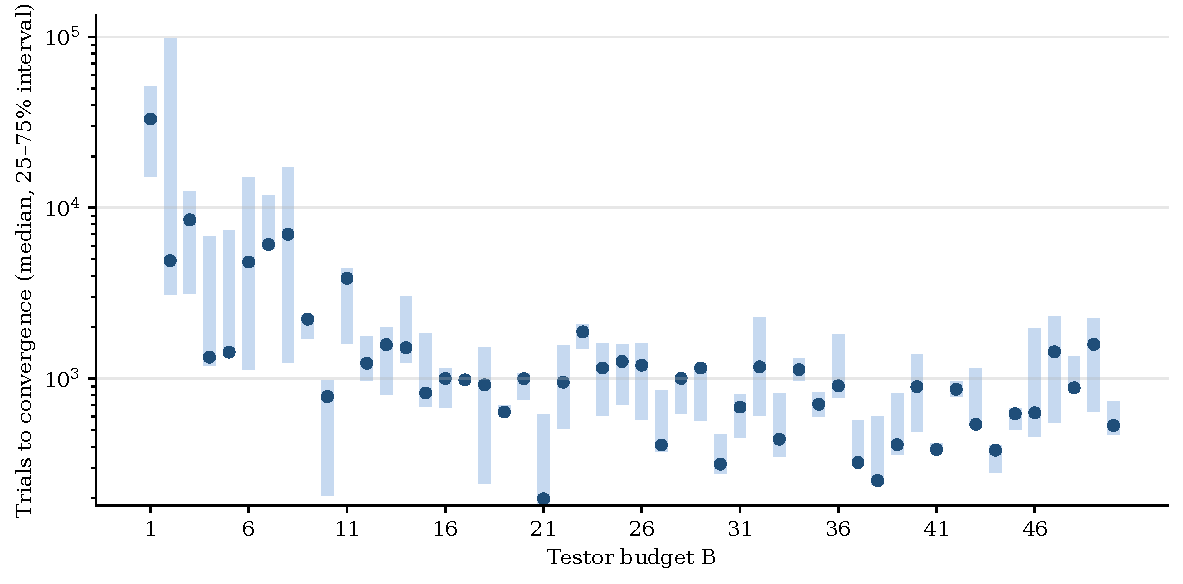
\includegraphics[width=0.8\linewidth]{images/trials.pdf}
  \caption{Median trials to convergence across budgets, with the 25th--75th percentile (IQR) band shown; the y-axis is log-scaled.}
  \label{fig:trial}
\end{figure}

%\subsubsection*{Scaling with Budget}

Based on the previous results, a budget of 20 appears sufficient for most of our purposes, offering comparable accuracy while requiring fewer computational resources than a budget of 50. To better understand the effect of the budget on convergence, we now revisit the \textsc{Sigma} benchmark, the only benchmark in our suite for which offline \testor with budget~20 requires more than 1,000 trials to converge. \textsc{Sigma} also has the largest exact count in the suite, at 1.7 million executions. 
Using this benchmark as a stress test, we study how the number of trials required for convergence varies with the budget. 
For each budget, we run \testor with five seeds and increase the trial cap until all seeds satisfy our convergence criterion or the cap reaches one million trials.


In Figure~\ref{fig:trial}, we plot the 25–75\% (IQR) band and mark the median explicitly. We observe that, as expected, larger budgets generally lead to more stable convergence. Some smaller budgets may still struggle to converge even after $10^5$ trials while larger budgets over 20 typically converge for all seeds within only a few hundreds trials. 
% This observation also supports the view that stochastic enumeration is effective at variance reduction: 
% for a fixed total amount of work, running \testor with budget~$k$ produces significantly more accurate estimates than running \testor with budget~$1$ for $k$ separate runs.
%
However, the pattern shown in the figure is not strictly monotone:  these irregular spikes are due to randomness under a finite number of seeds—at certain budgets we are simply ``unlucky.” In expectation over the randomization, increasing the budget can only improve, or at worst leave unchanged, the estimator’s performance.


%\subsection{Configuration~\ref{phase:trust-cost}: \jmc Cost Estimation }We now apply \testor to predict the cost of model checking.
%
%In this section, we specialize \testor to a concrete use case: estimating the cost of the model checker \jmc. This use case is particularly compelling, as model checkers have notoriously unpredictable runtimes, which can be extremely long even for small programs. Our experiments focus on evaluating how accurately our estimator approximates the cost induced by \jmc.

%As a potential application, a model checker could first run our estimator for a few hundred trials to obtain an estimate of how many execution graphs it will explore. During the actual verification run, it could then maintain a counter of graphs traversed so far and periodically report this count relative to the estimated total as a lightweight progress indicator.\subsubsection*{Cost Model}In estimating the cost of model checking, we consider not just the maximal executions but also other execution graphs constructed by the model checker.We add the following nodes and costs.\begin{description}   \item[\textbf{Inconsistent graphs:}] In estimating $C(P)$, we ignored execution graphs that are inconsistent in $\mathcal{D}(P)$. However, \jmc needs to construct these graphs, check consistency, and filter them.
%  Section~\ref{trust_sec} specifies the tree $\mathcal{D}(P)$ for a program $P$. 
%  \jmc explores $\mathcal{D}(P)$ in an optimal manner, but at additional cost: 
%  at each execution graph it explores not only all consistent partial orders, 
%  but also some inconsistent ones. Such costs in necessary to compute the transition relation of $\mathcal{D}(P)$. To model this cost, we represent inconsistent successors as leaves in the tree.\item[\textbf{Weights:}] Algorithm~K and Algorithm~S extend naturally to estimating the total weight of a weighted tree, instead of only counting leaves \cite{knuth75, vaisman2017}. This is crucial for designing an estimator of \jmc’s total cost: \jmc induces some cost over all execution graphs, not only to maximal ones. By estimating the total weight of the corresponding tree, we obtain a direct estimator for the total cost induced by \jmc. For our evaluation, we assign a uniform cost to every execution graph explored by \jmc. One can make this more precise, e.g., by assigning a cost proportional to the size of the graph.\item[\textbf{Blocked executions:}] Finally, we also represent blocked executions in the tree.
%As discussed, DPOR-based model checkers may traverse execution graphs in which some threads are permanently blocked, and these execution graphs can be either maximal or non-maximal. In our tree model, we also include the nodes corresponding to such blocked executions\end{description}\subsubsection*{Summary of results}In Table~\ref{tab:cost}, we repeat the Configuration~\ref{phase:acp} evaluation with budget~20 on the same benchmarks, and additionally include six benchmarks where \jmc explores many blocked executions, to estimate the cost. 
%% For clarity of presentation, we omit the input details of benchmarks previously presented. Our first observation is that \testor with a budget of 20 requires a similar number of trials to converge across most of the benchmarks presented earlier. The only exception is Sigma, where the success ratio fell from 1.0 to 0.6. The additional benchmarks are notably more challenging: \testor converged under all seeds on only 2 of 7 and failed to converge on 1. The average relative error increased by roughly an order of magnitude, yet remains within—or close to—the 20\% band.Another observation is that benchmarks with a similar number of complete executions can differ dramatically in the cost required to fully traverse their execution spaces. For example, incNTest and FineCounter have the same number of complete executions ($518400$), but incNTest has $683859$ total execution graphs, whereas FineCounter has $2191297$.This supports our conjecture that the total number of execution graphs is a better proxy for the cost of model checking than the number of complete executions alone.Overall, our experiments indicate that \testor is stable and robust for estimating the cost of model checkers, delivering accurate estimates with modest budgets and moderate numbers of trials across a diverse set of benchmarks.